 \begin{refsection}
 \chapter{Primary Contributions and Outlook}

For more than sixty years, scientists have been studying the molecular structure and function of voltage-gated sodium channels in order to better understand the basis for electrical signalling in living organisms. Our studies of ionic conduction, selectivity, gating, and leakage are significant contributions to this end. This research strengthens the link between the structural features of the voltage-gated sodium channel, such as the selectivity filter, intracellular gate, and voltage-sensors, to its functional properties for conduction, selectivity, and gating (Fig. \ref{fig:outlookFig1}). In this chapter, we summarize the contributions of this thesis; describing our primary results and the future research directions for each of the four main topics covered.

\begin{figure}[hp]
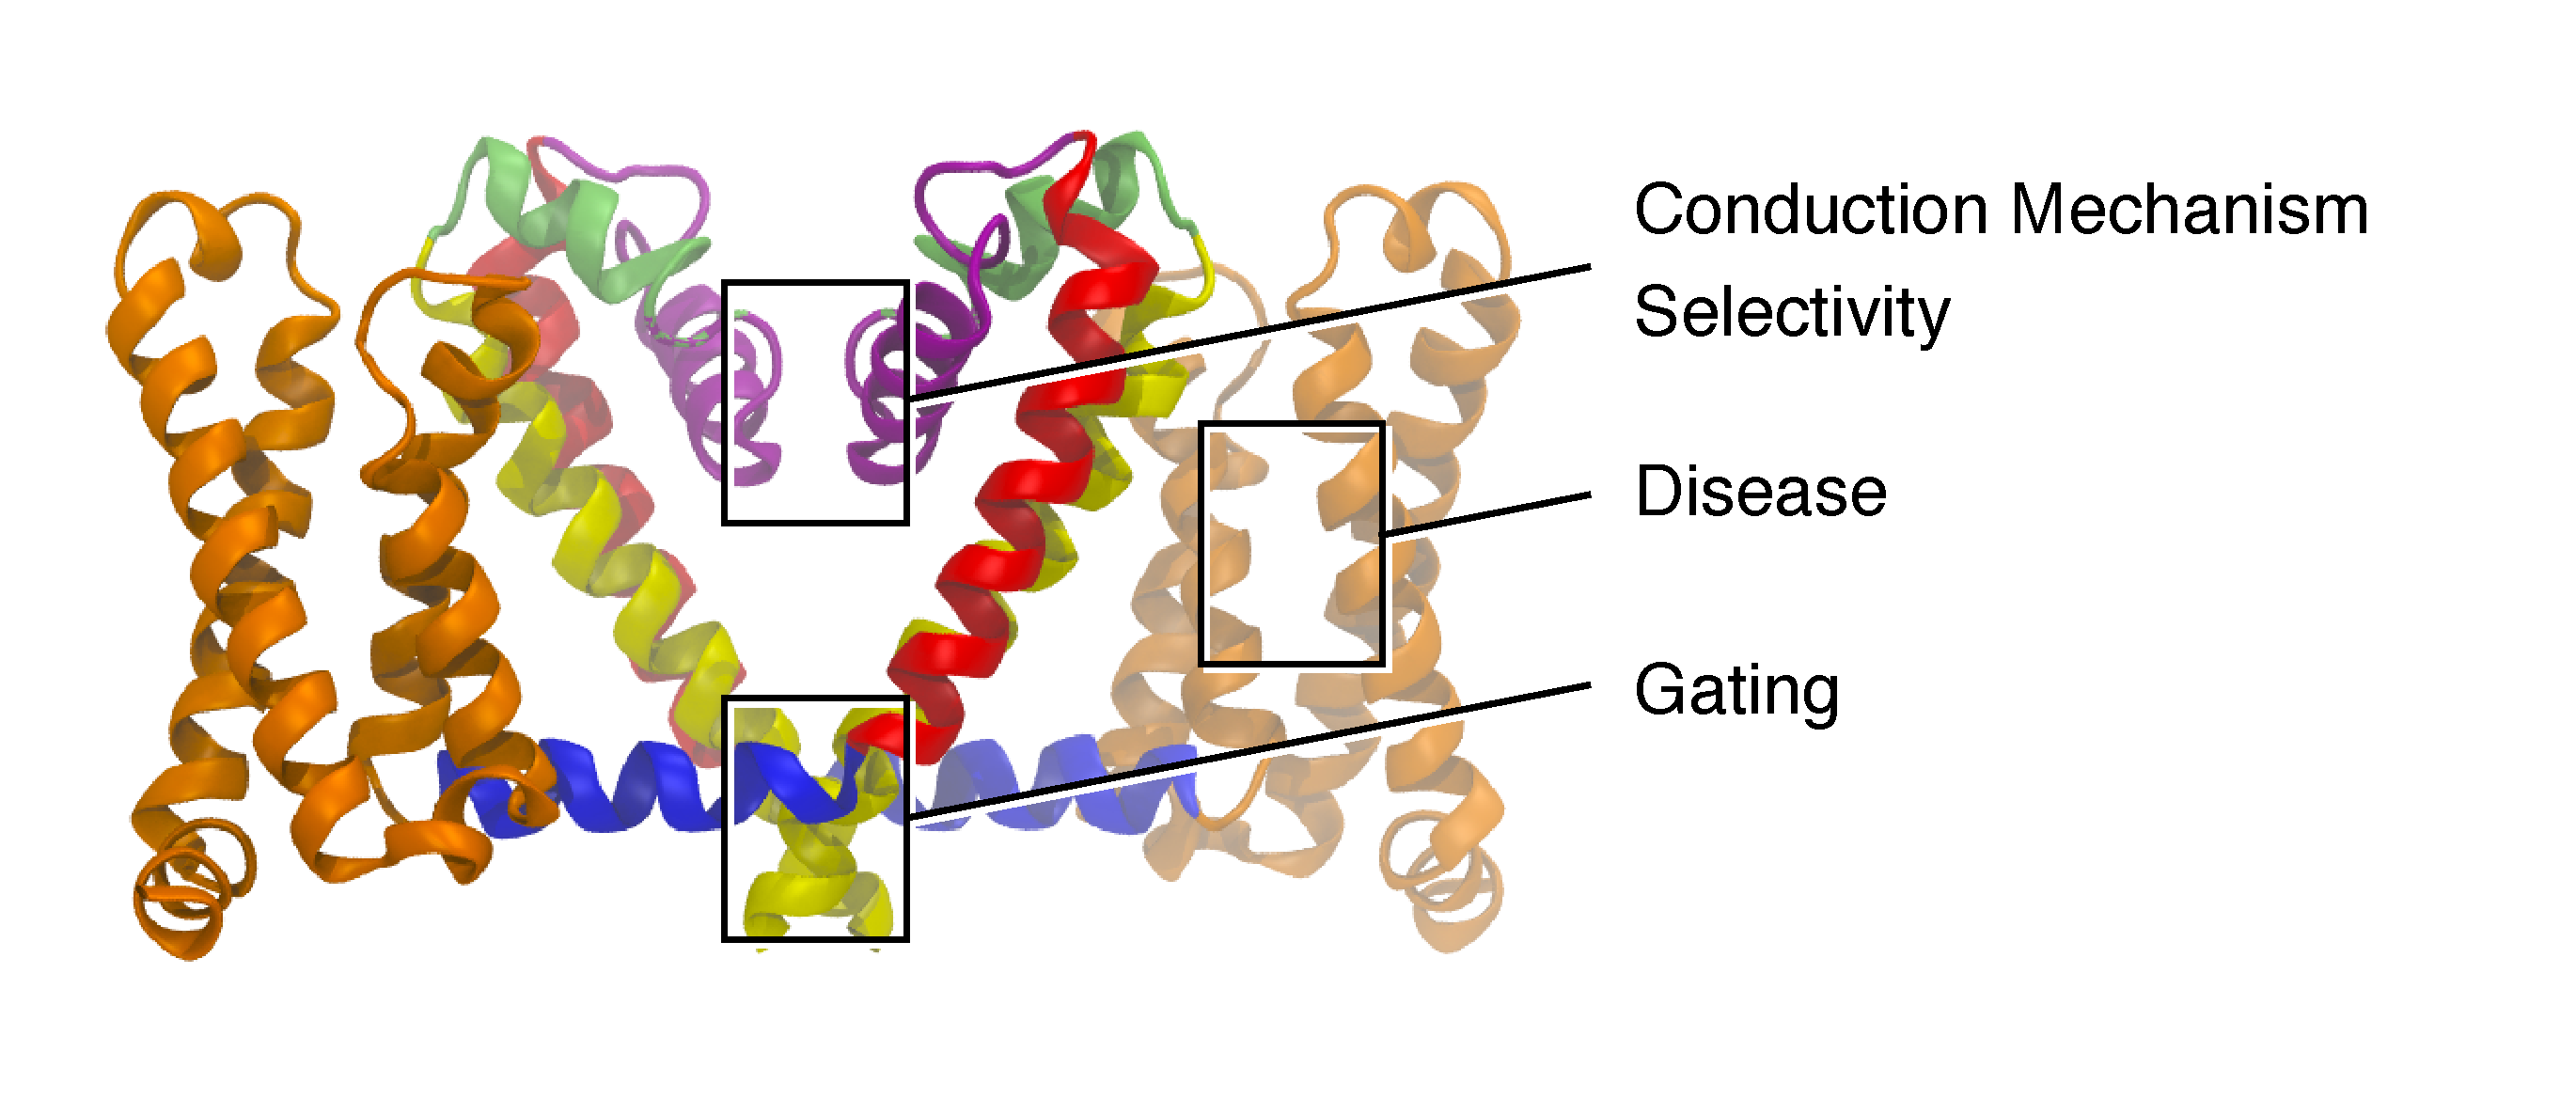
\includegraphics[width=1.0\textwidth]{outlook/outlookFig1}
\caption[Research contributions linking molecular structure to the function of Na\textsubscript{V} channels]{\textbf{Research contributions linked to the structure and function of Na\textsubscript{V} channels}. Molecular visualization of Na\textsubscript{V}Ab from the side. Voltage sensing domains (S1-S4 helix, orange), the S4-S5 linker (blue), the S5 helix (red), pore helices 1 and 2 (purple and green, respectively), and the S6 helix (yellow) are highlighted. Arrows indicate regions of the channel structure which are associated with research conducted in this thesis. Only two protomers of the tetrameric assembly are shown for clarity.}
\label{fig:outlookFig1}
\centering
\end{figure}

\section{Conduction}
%-Fixed binding sites, single-file conduction, solid knock-on mechanism, largely dehydrated ions, highly selective.
%Flexible binding sites, dual occupancy of sites, liquid knock-on mechanism, partially dehydrated ions, weakly selective

%At the molecular level, ion conduction can occur through numerous possible mechanisms; ranging from passive diffusion to an ATP-driven chemical process. A molecular model for ion conduction encapsulates this biophysical process and enables scientists to understand the free energy required for ion translocation. An accurate model provides a structural basis for understanding macroscopic functional properties of the channel such as the conductance rate. Having an accurate model enables the design of new experiments to investigate channel function and dysfunction. For example, in Na\textsubscript{V} channels, a molecular mechanism for conduction enables investigation of pore-blocking marine toxins (tetrodotoxin and saxitoxin) \cite{10.3389/fphar.2011.00071,Pennington:2018ud}, as well as antiepileptic, antiarrhythmic, and local anesthetic compounds \cite{Fozzard:2011tb,Bagal:2015ega}. 

%Electrophysiological methods can be used to obtain single-channel measurements of ionic conduction in Na\textsubscript{V} channels, with rates on the order of 10$^6$ ions per second \cite{Hille:1972wz}. Peak conduction occurs at membrane potentials close to 0 mV, suggesting that Na\textsubscript{V} channels can support conduction driven by concentration gradients alone, as well as a combined electrochemical gradient. An accurate model of conduction should qualitatively reproduce conduction rates for Na$^+$ at 0 mV, as well as the rates of other physiological cations like K$^+$.

Across diverse protein families, ion conduction has evolved to proceed through numerous mechanisms; ranging from passive diffusion to an ATP-driven chemical process \cite{Zheng:2015vj}. We performed an extensive study of Na$^+$ conduction in Na$_V$Ab revealing a novel molecular mechanism. Our work reveals that conduction through the SF occurs through a complex balance of forces arising from ion-ion, ion-water, ion-protein, and protein-protein interactions. Such factors have previously been described in the study of K$^+$ conduction in K$^+$ channels, but we note several distinct differences unique to bacterial Na$_V$ channels:
\begin{itemize}
\item \textbf{Hydration} Na$^+$ remains partially hydrated as it permeates the SF of Na$_V$Ab, whereas almost all water molecules are stripped from K$^+$ as it permeates K$^+$ channels.
\item \textbf{Binding modes} Na$^+$ can adopt multiple iso-energetic binding modes in the SF of Na$_V$Ab, accommodated by flexible glutamic acid sidechains, whereas K$^+$ adopts fixed binding modes, accommodated by relatively rigid cages of backbone carbonyls in K$^+$ channels. 
\item \textbf{Occupancy} Dual ion occupancy of binding sites, particularly near glutamic acid sidechains, is observed for Na$^+$ in Na$_V$Ab, whereas only single-file ion occupancy is observed for binding of K$^+$ in K$^+$ channels.
\item \textbf{Molecular mechanism} Na$^+$ conduction proceeds through a liquid-like energy landscape, resulting a soft `knock-on' mechanism, wherein a unitary ion conduction event can occur through either a 1-ion or 3-ion intermediate state (Fig. \ref{fig:outlookFig2} B). K$^+$ conduction proceeds through a solid-like hard `knock-on' wherein a unitary ion conduction event involves a `Newton's balls' mechanism (Fig. \ref{fig:outlookFig2} A).
\end{itemize}

Our simulations provide support for a novel cation channel conduction mechanism which couples rapid ionic diffusion to channel fluctuations within the SF. We developed a framework to test this molecular mechanism experimentally. Simulations of mutations to the hydrogen bonding network around glutamic acid sidechains within the SF reveal that mutagenesis has a direct effect on glutamic acid dunking and ionic conduction. In mutants that disfavour conformational dunking of glutamic acid sidechains, Na$^+$ conduction rates are expected to be lower, and in mutants that favour dunking, Na$^+$ conductance may be increased (up to the diffusion limit). Site-directed mutagenesis and electrophysiology can thus be used to validate our mechanism and determine the magnitude of this effect. Collectively, we present a novel mechanism of conduction in Na\textsubscript{V} channels which is in qualitative agreement with experiments, and leads to consequences that can be tested through experiments.

There are three primary research directions which should be investigated in order to extend the significance of our work on ionic conduction:
\begin{itemize}
\item \textbf{Accuracy}. To obtain quantitative predictions of conduction rates, additional experiments should be performed in order to investigate two sources of systematic error in our models. Firstly, the majority of our work on conduction was performed in a closed-channel model. Although the selectivity filter is unchanged in open and closed intracellular gate structures \cite{McCusker:2012di}, conduction rates should be computed using the number of cations crossing membrane in an open model rather than through the selectivity filter. Secondly, in order to compute conduction rates for K$^+$, additional experiments using quantum calculations should be performed to ensure that solvation of Na$^+$ and K$^+$ to carboxylate sidechains is accurately balanced with that of water molecules. These model parameters should be optimized within a confined system analogous to the chemical environment of a pore.
\item \textbf{Generality}. The molecular mechanism of conduction should be examined in non-bacterial Na\textsubscript{V} channels containing flexible sidechains. The EEEE ring is found in the selectivity filter of mammalian calcium channels Ca\textsubscript{V}1.1. The importance of our mechanism will be significantly increased if it is found that channel fluctuations within the selectivity filter can facilitate rapid conduction of Ca$^{2+}$ in addition to Na$^+$.
\item \textbf{Robustness}. Additional simulations should be conducted at a range of physiological conditions in order to confirm that our proposed mechanism is unchanged. All simulations in this work were performed at a membrane potential of 0 mV, but conduction rates should follow a linear relationship under a range of external applied voltages. This will lead to a proper estimate of ionic conductance and enable better comparison to experiment.
\end{itemize}

\begin{figure}[hp]
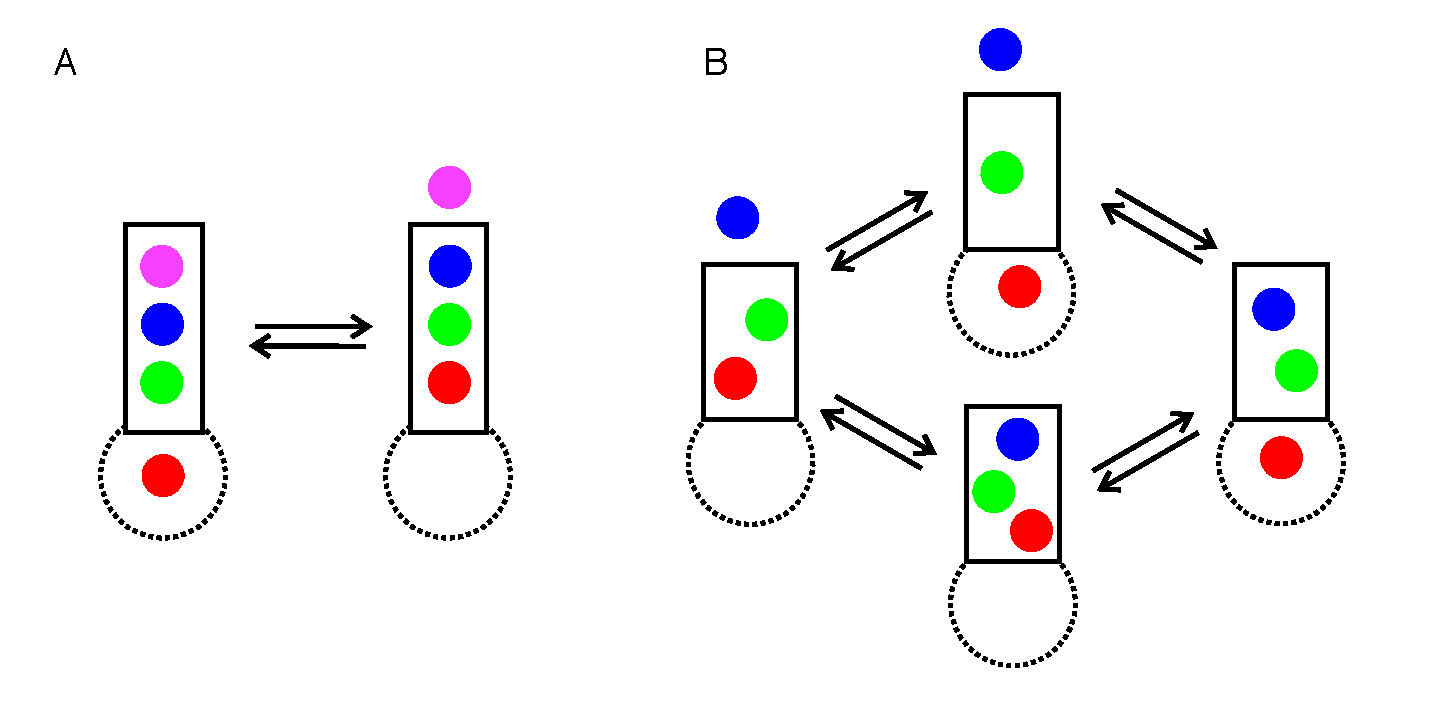
\includegraphics[width=1.0\textwidth]{outlook/outlookFig2}
\caption[Comparison of K$^+$ and Na$^+$ Channel Ion Conduction Mechanisms]{\textbf{Comparison of K$^+$ and Na$^+$ Channel Ion Conduction Mechanisms}. Schematic representation of ionic conduction in (\textbf{A}) K$^+$ and (\textbf{B}) N$^+$ channels. Colored circles (red, green, blue, magenta) represent ions, the rectangle represents the selectivity filter (SF), and the dotted circle represents the central cavity of the channel. Arrows denote an interconversion between channel occupancy states and describe unitary ionic conduction events moving from left to right.}
\label{fig:outlookFig2}
\centering
\end{figure}

\section{Selectivity}

%Channels intrinsically select for specific ions over a range of small compounds and metabolites inside and outside of the cell. How channels achieve ion selectivity is a fundamental question in the study of these proteins, and it is still largely unknown\cite{Andersen:2011ty}. Understanding how these proteins are selective would enable major advancements in the study of a larger set of biological processes driven by ion-protein interactions, which includes protein folding/stability \cite{Baldwin:1996to,Hribar:2002hq}, binding \cite{Lundback:1996fd}, activity \cite{Glusker:1991ux}, and regulation \cite{Neale:2015ee}. Beyond addressing the basic science of protein function, a molecular mechanism for selectivity is integral to the design of new synthetic ion channels and biologically-inspired nanodevices that could act as sensors or filters \cite{He:2013it,Rollings:2016hz}. 

%Our work sheds light on the molecular mechanism of selectivity in a class of channels that has evolved to function with relatively weak selectivity ($\sim$100 times less selective than some K$^+$ channels). An accurate molecular model for selectivity should reproduce the relative permeability of ions, and be in agreement with selectivity altering mutations and conditions. In the case of bacterial Na\textsubscript{V} channels, the ratio of conductance or occupancy of binding sites should be in favour of Na$^+$ over K$^+$ by a factor of $\sim$10, even at 0 mV membrane potentials \cite{Payandeh:2012ib}. It is known that the EEEE to DDDD mutation in the SF and low pH conditions can reduce selectivity for Na$^+$ over K$^+$ \cite{FinolUrdaneta:2014bz}, and a robust model should qualitatively reproduce these results. 

The molecular mechanism for ion selectivity is a fundamental question in the study of channels, and remains poorly described in even the most well-studied K$^+$ channels \cite{Andersen:2011ty}. We performed a large-scale computational study of Na$^+$ and K$^+$ selectivity in Na$_V$Ab using both pure cation and mixed cation salt concentrations. This resulted in the largest simulation dataset generated to investigate selectivity in ion channels to date, which affords us enough statistical power to distinguish characteristic differences in conduction mechanisms (though systematic force field errors may still be present). Simulations reveal a complex and strikingly subtle mechanism wherein glutamic acid sidechains create a diffusive and liquid-like free energy landscape for Na$^+$, but not for K$^+$. The primary free-energy barrier for K$^+$ permeation in the SF coincides with a region where the coordination of K$^+$ to water molecules reaches a maximum. This supports the hypothesis that the intrinsic geometric properties of the SF, the size of the permeant cations, and the conformational flexibility of sidechains, are the primary factors governing Na$^+$ selectivity in Na$_V$Ab. Additionally, our models qualitatively reproduce expected selectivity ratios for Na$^+$ over K$^+$, as well as the expected loss of selectivity through modifications of the Glu sidechains (Glu to Asp SF mutation, and lowering of pH) \cite{FinolUrdaneta:2014bz}. %Although the mechanism for K$^+$ selectivity in K$^+$ channels is still under debate, it is known that thermodynamic factors like conformational flexibility and structural strain, as well as kinetic factors related to the multi-ion nature of the pore are important \cite{Roux:2017bs}. Similarly, each of these factors plays an important role in selectivity for Na\textsubscript{V} channels, where the multi-ion nature of the pore is even more significant due to the large number of ionic configurations possible within the SF. 

Based on our findings, additional studies should be performed in order to investigate remaining open questions related to selectivity:
\begin{itemize}
\item \textbf{Validation}. Our simulations have only been used to examine selectivity from a thermodynamic perspective. Additional simulations should be performed to compute observables like the reversal potential and the ratio of conductance that are more directly comparable to electrophysiological measurements. For this, a stable open-state model of the channel must be established and new simulations must be performed under a range of external applied membrane potentials.
\item \textbf{Effect of SF Conformation}. Na$_V$Ab is reported to adopt an inactivated state of the SF, but the role of this state in gating is unknown \cite{Payandeh:2013ex}. Additional work must be perform to determine if the conformation of the SF is perturbed enough to alter conduction and selectivity in a manner similar to the collapsed SF of K$^+$ channels \cite{Zhou:2001vo}.
\item \textbf{Generality}. It is not known if our mechanism for selectivity applies to other sodium-selective channels like Na\textsubscript{V}1.4 and Na\textsubscript{V}1.7, where the SF contains the sequence DEKA rather than EEEE. Our model suggests that carboxylate sidechains function to catalyze conduction and support a diffusive free energy landscape for Na$^+$. The overall reduction of negative charge within the SF of mammalian channels and the critical importance of the Lys suggests that our model of Na$_V$ channel selectivity may need to be revised \cite{Ahern:2016jf,Heinemann:1992ep}. Furthermore, the existence of Ca$^{2+}$ selective channels with sequence EEEE further stresses the importance of testing the generality of our mechanism in homologous channels.
\end{itemize}

\section{Gating}
% Gating
%Ion channels have evolved diverse mechanisms for regulating conductance \cite{GoldschenOhm:2017hx}. In voltage-gated cation channels, conductance in the pore domain is regulated by opening and closing of the intracellular gate. The capability of both Na\textsubscript{V} and K\textsubscript{V} channels to adopt multiple conformations is integral to this process. In a more general sense, gating is a form of coupled conformational change due to a physiological stimulus, and thus its study has implications for understanding allosteric processes in a wide range of membrane proteins. In Na\textsubscript{V} channels, developing a molecular mechanism for gating has potential for providing structural insights that may assist in pharmacology and treatment of inherited diseases. There have been recent successes in developing small molecules and peptides that modulate gating through binding to the voltage sensors of Na\textsubscript{V} channels rather than pore blockage \cite{Ahuja:2015co,Payandeh:2018bb}.

%The molecular mechanism of voltage-dependent gating in Na\textsubscript{V} channels is not well described. Studies of K$^+$ channels suggest that activation involves conformational change in the voltage sensor, followed by movement of the S4-S5 linker and the intracellular gate formed by the S6 helices \cite{Blunck:2012fj}. Key residues involved in mammalian Na\textsubscript{V} channel gating were identified though experiments, and used to propose a model involving the movement of rigid segments connected by elastic hinges to open the channel \cite{Muroi:2010do}. Crystallographic structures of the bacterial Na\textsubscript{V} channel with pore domain S6 helices in both closed and open conformations appear to support this finding. An iris-like dilation of the S6 gate appears to be wide enough to support the permeation of cations but requires validation to determine if the constriction is indeed permeable. Simulating the dynamics of the entire open-closed-inactivated gating process is of highest value for the study of ion channel function \cite{Bagneris:2014eh}, but unfortunately this occurs on a timescale that is prohibitively long for modern supercomputers. Rather, we are interested in understanding the molecular mechanism of ion conduction within the pore in the region of the intracellular gate, and to develop a model for how gating is achieved at this location.

%Our structure and simulations are in good agreement with solvent accessibility studies \cite{Oelstrom:2014ky}. 

Ion channels have evolved diverse mechanisms for regulating conductance \cite{GoldschenOhm:2017hx}. We presented the first direct comparison of an open-state and closed-state conformation of the bacterial channel Na$_V$Ab. By performing molecular simulations, we confirmed that the open-state is permeable to cations and we were the first to propose a mechanism by which Na$^+$ conduction is regulated at the intracellular gate through a hydrophobic gating model \cite{Aryal:2015ge}. We observed fluctuations in the pore diameter, hydration, and free energy of ion permeation at the intracellular gate. In our model, a relatively subtle rearrangement of pore helices is sufficient to mediate opening and closing of the gate through modulation of a hydrated (wetted) or dehydrated (dewetted) state in the constriction. We determined that the wetted state can be promoted by making a double alanine mutation for the pore lining residues in the intracellular gate, which can be utilized as a stable open-state model for subsequent studies of conduction and selectivity. There are interesting implications of our findings for the interpretation of tunnels and pockets in static structures of proteins, which should not be presumed to be continuously hydrated or dehydrated without additional functional analysis.

Several studies are required to develop a more comprehensive model for gating in Na\textsubscript{V} channels:
\begin{itemize}
\item \textbf{Stability}. An accurate computational model for the physiological open-state is characterized by stabilization of the intracellular gate in a hydrated and ion-permeable state. Additional research should be performed using a structure of Na\textsubscript{V}Ms with an interaction motif proposed to stabilize the open state \cite{Sula:2017jx}. Similarly, it would be useful to determine if an even more open state, such as those observed in K$^+$ channels \cite{Cuello:2010gi}, can be obtained for Na\textsubscript{V}Ab using computational methods. A stable open-state model will permit extensive studies of conduction and selectivity in closer agreement to electrophysiological data.
\item \textbf{Helix Kinking}. Early models of cation channel gating are supportive of a putative hinge in the S6 helices \cite{Jiang:2002fx,Zhao:2004vo,Shafrir:2008ic}. A kink is observed in the S6 helix of our open state, but additional simulations should examine the relationship between this structural perturbation in the helix and the intracellular gate diameter. Previous molecular simulations suggest that this kinking may act as an inactivation mechanism \cite{Boiteux:2014ut}. In addition, a conserved asparagine near the putative gating-hinge position which makes contacts with the S4-S5 linker should be investigated to understand its functional importance in gating \cite{OReilly:2017ur}.
\item \textbf{Electromechanical Coupling}. To develop a more comprehensive molecular mechanism of Na\textsubscript{V} channel gating, simulations must be performed with external applied voltage. Long timescale simulations were successful for inducing conformational change in the voltage sensor and activation gate of a K$^+$ channel to propose two possible electromechanical gating mechanisms \cite{Jensen:2012ee,FernandezMarino:2018vw}. Further work should be performed to determine which model may apply to bacterial Na\textsubscript{V} channels.
\end{itemize}


\section{Disease}
% Disease
%Mutations in human genes encoding Na\textsubscript{V} channel subtypes have been linked to channelopathies such as epilepsy, cardiac arrhythmias, and chronic pain syndromes \cite{Ashcroft:2000ts,Catterall:2008bz,JurkatRott:2010eo}. Despite establishing strong genetic correlations between single-point mutations and disease phenotypes, a lack of structural data for mammalian channels prevents the determination of the molecular basis for these channel dysfunctions. At an atomistic level, disease can result from impairment of any of the functional properties described above, including conduction, selectivity, and gating. Ultimately, these perturbations all modify Na$^+$ conduction, resulting in abnormal levels of Na$^+$ or K$^+$ which affect cell excitability. Structural models can be used as the basis for rational drug design for correcting these gain-of-function or loss-of-function mutations. 

%Na\textsubscript{V} and K\textsubscript{V} channels tightly regulate the concentration of Na$^+$ and K$^+$ to permit electrical signalling. Disruption of this balance can result in devastating neuromuscular disorders. Here we focus on a type of inherited skeletal muscle disease characterized by temporary attacks of paralysis, called hypo- and normokalaemic periodic paralysis. Mutations in the arginine gating charges of the Na\textsubscript{V}1.4 channel voltage sensor S4 helix cause state-dependent leakage of ions which is referred to as the gating pore current \cite{Sokolov:2005ec,GamalElDin:2014gu}. Although multiple single point mutations were linked to this disease, its pathogenic mechanism was not understood at the atomistic level in Na\textsubscript{V} channels.

Mutations in human genes encoding Na\textsubscript{V} channel subtypes have been linked to channelopathies such as epilepsy, cardiac arrhythmias, and chronic pain syndromes \cite{Ashcroft:2000ts,Catterall:2008bz,JurkatRott:2010eo}. We contributed to understanding of the skeletal muscle disease `periodic paralysis' which is linked to mutations in the human Nav channel voltage sensing domains. We were the first to present a structural mechanism for this disease, based on a combination of crystallographic structures and molecular dynamics simulations. The structure of a mutant voltage sensor `R3G' linked to this disease revealed no backbone conformational change compared to the wildtype structure, and motivated the use of simulations to investigate hydration and Na$^+$ conduction in the voltage sensor. A decrease in free energy barrier opposing Na$^+$ conduction was observed at the hydrophobic constriction of the R3G voltage sensor when compared to the wildtype, which also coincides with the position occupied by the R3 side chain, and a region requiring high coordination of Na$^+$ to water molecules. This finding is in agreement with the electrophysiological measurements for the activated R3G voltage sensor. 

Employing the same computational approach used in this study, several new experiments should be performed to further understand and treat this disease:
\begin{itemize}
\item \textbf{Mammalian model}. Experimental work confirms gating pore currents in the bacterial voltage sensor, but it is not known if the same mechanism of leakage occurs in the human Na\textsubscript{V}1.4 channel since structures of this protein are not available. Homology models of human Na\textsubscript{V}1.4 should be created and validated using a moderate resolution cryo-EM structure of the electric eel Na\textsubscript{V}1.4 channel \cite{Yan:2017kda}, and this study should be repeated.
\item \textbf{Robustness}. The generality of our mechanism should be tested by examining multiple missense mutations that can cause hypokalaemic or normokalaemic periodic paralysis \cite{JurkatRott:2012kv,Moreau:2014jy}. In this work we performed simulations of the most dramatic mutation of arginine to glycine, but future work should investigate the Gln and Trp at the R3 position \cite{Jiang:2018ga}. Similarly, using a model of the VSD in the resting state, the Arg to Trp, Gly, Gln, or Ser mutation should be made at the R2 position. Collectively, these simulations should provide a more comprehensive understanding the molecular basis for periodic paralysis, and test the generality of our findings in Na\textsubscript{V}Ab.
\item \textbf{Drug Design}. A guanidinium binding site was identified in the resting state of R2S, which was sufficient to block gating pore currents. Computational studies may be performed to assist in the development of drugs that selectively bind the voltage sensor and mimic guanidinium for the treatment of periodic paralysis. These drugs must be optimized to not impact the delicate gating cycle of Na\textsubscript{V} channels.
\end{itemize}

\section{Outlook}

The bacterial voltage-gated sodium channel has immense utility in the study of ion channels and membrane proteins as a whole. Experiments, both computational and experimental, provide us with novel insights into the role of channel fluctuations in conduction and selectivity, new perspectives on channel regulation through gating, and a structural basis for diseases linked to ion leakage. As new and innovative methodologies are applied to sodium channels, conventional paradigms for channel structure and function are revised, expanding the scope and complexity of what channels have evolved to achieve within living organisms. The computational approaches we employed to investigate the voltage-gated sodium channel are no exception, enabling us to propose new experimentally testable hypotheses linking structure and function. As computational methods improve, higher accuracy models will be constructed that can be used to access longer timescale processes. With such models we may eventually be able to simulate the dynamics of the entire open-closed-inactivated gating cycle, and use this to compare more directly with experiments to understand the role of ion channels in human health and disease.

Throughout this thesis we observed multiple instances of mechanisms that were in stark contrast with traditional thinking. Much of our understanding of channels is based on studies of K$^+$ channels, and proposed mechanisms reflect that bias. Even so, it is particularly remarkable that we observe contrasting molecular mechanisms given how Na$^+$ and K$^+$ channel structures are so similar in overall topology and structure. There is no question that as more cation channels structure are discovered and structurally characterized, that again, many of the mechanisms proposed in this work will be called into question and revised to fit new data. As with all areas of biology, ion channels are capable of staggering complexity, and rich multidisciplinary studies are crucial to uncovering their mystery. 
 
 \printbibliography[heading=subbibnumbered,title={References}]
%\printbibliography[heading=subbibliography]
\end{refsection}
